
\section{Part B}


%%%%%%%%%%%%%%%%%%%%%%%%%%%
\subsubsection*{Problem 3}
%%%
%%% Ameen (example 3.3, pg 50)
%%%
An ice plant operates on the ideal vapour-compression cycle with superheated state using refrigerant fluid R134a.  The refrigerant enters the compressor as saturated vapour at 0.15 MPa and leaves the condenser as saturated liquid at 0.7 MPa.  Water enters the refrigerator cavity at 30$^{\text{o}}$C and leaves as ice at -5$^{\text{o}}$C. For an ice production rate of 10 kg per hour, determine the power input to the ice plant and the COP of the cycle. Also, sketch the $PH$ and $TS$ diagrams. Specific heats of ice and water are 2.1 and 4.18 kJ/(kg.K), respectively, and the latent heat of fusion of ice is 334 kJ/kg. Repeat the same procedure for ammonia and propane as refrigerat fluid. 

{\it Hint: This problem was fully solved in Tutorial 4, but here you need to generate an algorithm to solve a generic vapour-compression refrigeration cycle. Also for the thermodynamic properties, you should either (a) use external public libraries or (b) produce libraries based on spline-based lookup tables.}


 

%%%%%%%%%%%%%%%%%%%%%%%%%%%
\subsubsection*{Problem 4}
%%%
%%% Ameen (example 3.3, pg 50)
%%%
A Thermal engineer is hired to design coupled steam-power and refrigeration plants (Fig.~\ref{Ex14:Fig}). The thermal plant (I) operates 100 kg/h steam in 3-turbines reheat Rankine cycle with initial conditions and efficiencies described in Tables \ref{Ex14:Tab1} and \ref{Ex14:Tab2}. 0.1$\%$ of the power generated by the set of turbines in {\bf I} is used in the compressor of the refrigeration unit {\bf II}. The refrigeration system operates with a working fluid, $\mathcal{X}$. Tasks:
\begin{enumerate}
\item Calculate the enthalpies of all stages assuming $\mathcal{X}=\left\{\text{Ammonia and R-134a}\right\}$. 
\item For both cases, calculate the mass flow rate of the refrigerant fluid and the refrigerant capacity. 
\item Calculate the net work for the thermal cycle {\bf I} $\left(\displaystyle\frac{\dot{W}_{\text{cycle}}}{\dot{m}_{\text{water}}}\right)$ and the power produced by the set of turbines $\left(\dot{W}_{c}\right)$.
\end{enumerate}

{\it Hint: This problem is similar to Question 14 in Tutorial 4, but here you need to generate an algorithm to solve the coupled generic thermal power and vapour-compression refrigeration cycle. Also for the thermodynamic properties, you should either (a) use external public libraries or (b) produce libraries based on spline-based lookup tables.}



\begin{table}[h]
\begin{center}
\begin{tabular}{ || c || c | c ||}
\hline\hline
{\bf Flow}& {\bf Pressure}  &  {\bf Temperature}    \\
          & {\bf (bar)}     & {\bf ($^{\text{o}}$C)}       \\
\hline\hline
{\bf 1}   &   200.0         &      600                \\
{\bf 2}   &   5.0           &       --                  \\
{\bf 3}   &   5.0           &      240                 \\
{\bf 4}   &   1.0           &      --                     \\ 
{\bf 5}   &   1.0           &    99.63                    \\ 
{\bf 6}   &   0.23          &      --                     \\
{\bf 7}   &   --          &      --                     \\              
{\bf 8}   &   --           &      --                        \\
\hline \hline
{\bf 9}   &   2.0           &      --                    \\
{\bf 10}  &  16.0           &     --                     \\ 
{\bf 11}  &  --         &     --                    \\
{\bf 12}  &   --          &    --                     \\ 
\hline\hline
\end{tabular}
\end{center}
\caption{Information on the steam-power and refrigeration cycles.}\label{Ex14:Tab1}
\end{table}



\begin{table}[h]
\begin{center}
\begin{tabular}{||c | c c c c | c||}
\hline\hline
               &  {\bf Turbine 1} & {\bf Turbine 2}  & {\bf Turbine 3}  & {\bf Pump}  & {\bf Compressor}\\
{\bf Efficiency}&    0.88          &   0.85           &     0.85         &  0.92      &  1.00           \\
\hline\hline
\end{tabular}
\end{center}
\caption{Efficiencies of the equipment used in the coupled units.}\label{Ex14:Tab2}
\end{table}



\begin{figure}[h]
\begin{center}
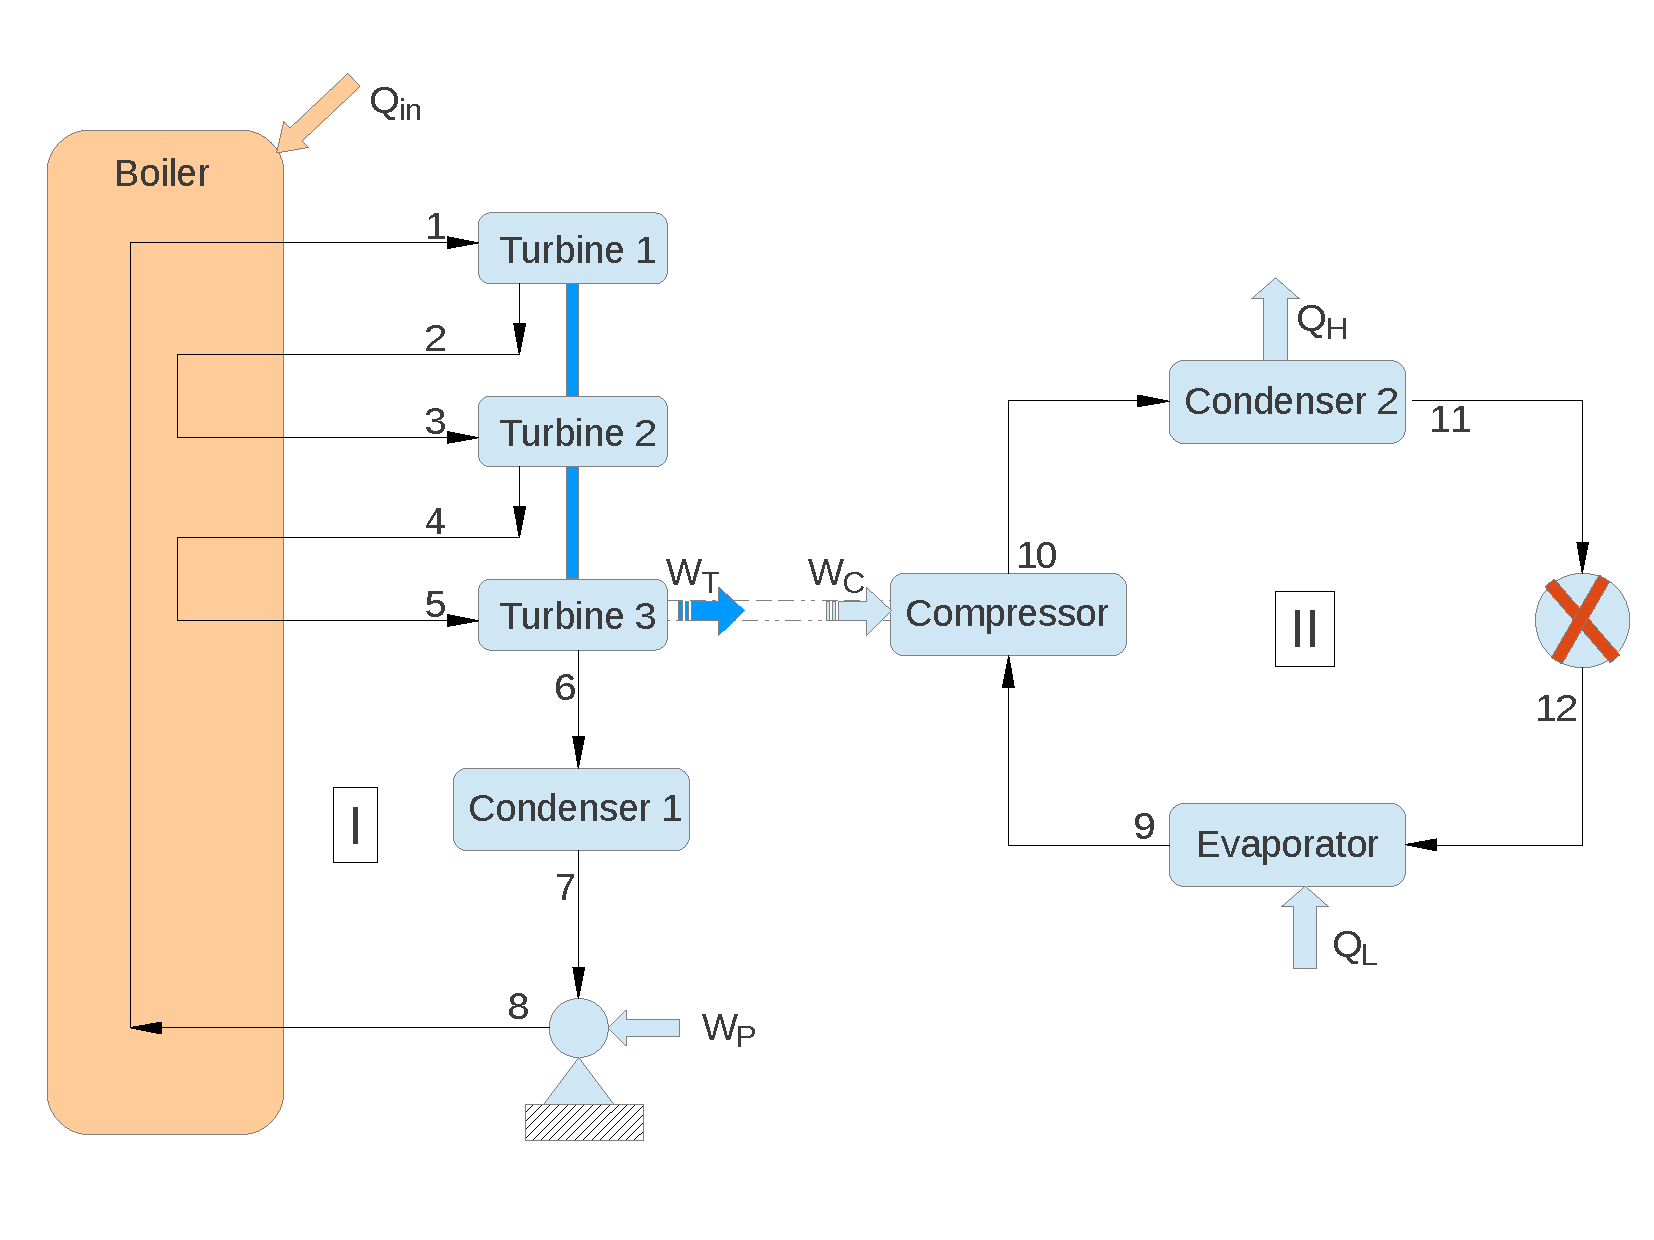
\includegraphics[width=16.0cm,height=12.0cm]{../Module_04/Pics/Overview_Refrig43}
\end{center}
\caption{Coupled reheat Rankine steam and reversed-Rankine refrigeration units.}\label{Ex14:Fig}
\end{figure}

